\documentclass{article}
\usepackage[english]{babel}
\usepackage{fancyhdr}
\usepackage{enumitem}
\usepackage{listings}
\usepackage{tikz-qtree}
\usepackage{tikz-qtree-compat}

\usepackage[lastexercise,answerdelayed]{exercise}
%DeclareCaptionType{mytype}[Typename][List of mytype]
%\newenvironment{myenv}{}{}

\tikzset{edge from parent/.append style={->}}

\newcommand\ExTitle{The Lambda Calculus}

\newcommand\fullExTitle{Exercises \\ \ExTitle }
\newcommand\footerExTitle{\ExTitle -\  Exercises }

\pagestyle{fancy}
\fancyhead{} % clear all header fields
\renewcommand{\headrulewidth}{0pt} % no line in header area
\fancyfoot{} % clear all footer fields
\fancyfoot[LE,RO]{\thepage}           % page number in "outer" position of footer line
\fancyfoot[RE,LO]{\footerExTitle} % other info in "inner" position of footer line

\begin{document}
\begin{Huge}
	\begin{center}
	\fullExTitle
	\end{center}
\end{Huge}
\begin{Exercise}
Write out lambda calculus trees for the following expressions.
\begin{enumerate}
\item $\lambda x.\lambda y.xy $
\item $\lambda x..\lambda y.xy.\lambda z.yz$
\item $\lambda x.(.\lambda y.xy)(.\lambda z.yz)$
\end{enumerate}
\end{Exercise}
\begin{Exercise}
Write out the equivalent lambda calculus expression for the following trees.

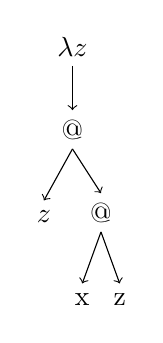
\begin{tikzpicture}
\Tree [.$\lambda z$   [.$@$ $z$ [.$@$ x z ]  ] ]
\end{tikzpicture}
%https://pages.github-dev.cs.illinois.edu/cs421-haskell/web/handouts/lambda-calculus-activity.pdf
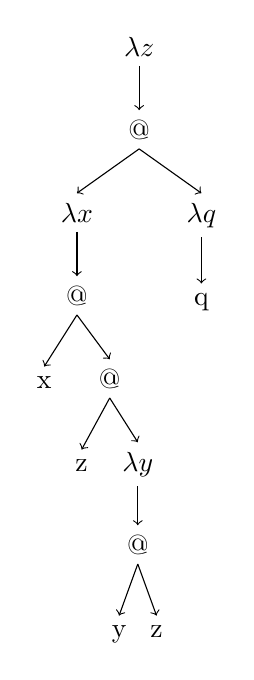
\begin{tikzpicture}
\Tree [.$\lambda z$  [.$@$  [ .$\lambda x$ [ .$@$ x [.$@$ z [.$\lambda y$   [.$@$ y z   ]] ]]]   [.$\lambda q$ q   ]  ] ]
\end{tikzpicture}
\end{Exercise}
\begin{Exercise}
Find the free variables 
What are the free variables? To which lambdas are bound variables bound? 

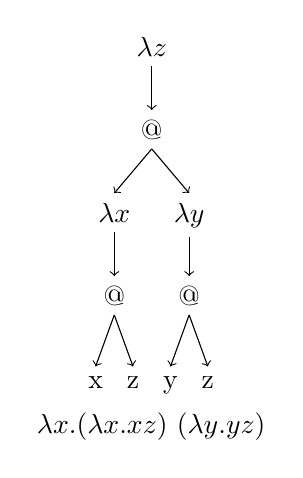
\begin{tikzpicture}
\Tree  [.$\lambda z$   [.$@$   
            [ .$\lambda x$
                    [ .$@$ x  z ] ] 
             [.$\lambda y$  
                    [.$@$  y z ] ]     ]
            ]
\node[below]at(current bounding box.south){ $\lambda x$.($\lambda x. xz$) ($\lambda y.yz$)   }  ;                      
\end{tikzpicture}
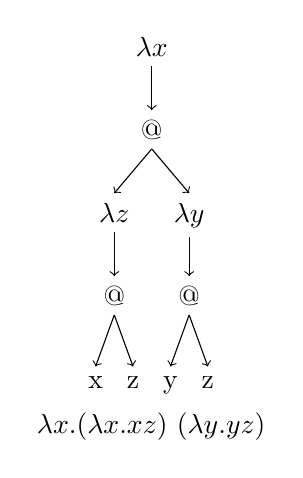
\begin{tikzpicture}
\Tree  [.$\lambda x$   [.$@$   
            [ .$\lambda z$
                    [ .$@$ x  z ] ] 
             [.$\lambda y$  
                    [.$@$  y z ] ]     ]
            ]
\node[below]at(current bounding box.south){ $\lambda x$.($\lambda x. xz$) ($\lambda y.yz$) } ;                    
\end{tikzpicture}
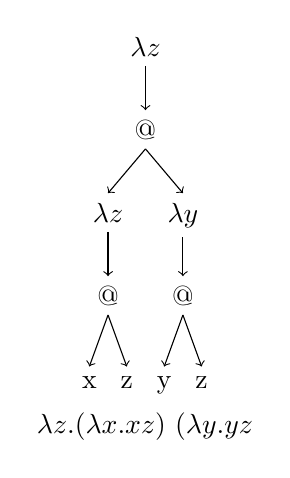
\begin{tikzpicture}
\Tree  [.$\lambda z$   [.$@$   
            [ .$\lambda z$
                    [ .$@$ x  z ] ] 
             [.$\lambda y$  
                    [.$@$  y z ] ]     ]
            ]
\node[below]at(current bounding box.south){$\lambda z$.($\lambda x. xz$) ($\lambda y.yz$};
\end{tikzpicture}
\end{Exercise}
\begin{Exercise}
Using $\beta$ reduction etc., rewrite these expressions in normal form.
\begin{enumerate}
\item $(\lambda x.x) y$
\item $(\lambda x.x z) (\lambda y.y)$
\item $(\lambda x.x (\lambda x.y)) (\lambda z.z)$
\item $(\lambda x.(\lambda y.x)) y (\lambda z.z))$
\item $(\lambda x.x x) (\lambda x.x x)$
\end{enumerate}
\end{Exercise}

\end{document}
